% This is a template for your written document.
%
% To compile using latexmk on the command line, run the following: 
% latexmk -pdf main.tex

\documentclass[12pt]{article}
\usepackage{setspace}
\singlespace
\usepackage[left=1in,right=1in,top=1in,bottom=1in]{geometry}
\usepackage{graphicx}

\title{\textbf{Multistep Synthesis Tool for Organic Chemistry Education}}
\author{Raelyn Brooks}

\begin{document}

\maketitle
 
\indent 
Organic chemistry has long been considered one of the most difficult undergraduate courses, with national failure rates often exceeding 50 percent. 
Among the challenges faced by students, multistep synthesis stands out as a major stumbling block. Success in synthesis problems requires balancing starting materials, reagents, intermediates, conditions, and stereochemistry, all while reasoning backwards (retrosynthesis) and forwards (reaction progression). 
Students often describe synthesis as a "black box": they know reactions individually, but cannot connect them into coherent strategies.
The purpose of this project is to design and implement an interactive software system that teaches multistep synthesis through decision trees and constraint satisfaction techniques. By breaking synthesis into a sequence of guided yes/no decisions, the system will reinforce fundamentals and provide educational feedback at each step. 
While professional chemistry tools exist—such as ChemDraw or Reaxys--these platforms are not designed for novice learners. This project fills the gap by prioritizing transparency, interpretability, and pedagogy over raw prediction power.
\\
\indent 
A number of research directions inform this project. From a computer science perspective, foundational graph algorithms are necessary for representing molecules and reactions as nodes and edges \cite{clrsAlgorithms}. 
This graph-based structure underpins most cheminformatics systems. On the theoretical side, Gale, Lobski, and Zanasi \cite{10.1016/j.tcs.2025.115084} propose a categorical model of organic chemistry, treating molecules as objects and reactions as morphisms. 
Their framework offers a formal way of reasoning about transformations, which can guide the development of rule-based synthesis logic. Decision trees provide a natural mechanism for structuring synthesis pathways.O’Sullivan, Ferguson, and Freuder show how decision trees can boost the efficiency of constraint satisfaction problems (CSPs) by reducing the search space and pruning infeasible solutions. 
\cite{10.1109/ICTAI.2004.38} Similarly, Shati, Cohen, and McIlraith demonstrate how decision trees can be combined with constraints to produce interpretable and accurate models. This is essential for an educational setting, where students must understand why a particular path works or fails. \cite{10.24963/ijcai.2023/225}
\textit{Decision trees with short explainable rules} further emphasize explainability by introducing methods for building decision trees with short, clear rules, making them particularly well suited for teaching environments. \cite{10.1016/j.tcs.2025.115344}
\\
\indent
Finally, the software must rest on an optimized data backbone. Reniers present schema recommender systems for document databases, which can be adapted to the chemical context. Their work highlights how workload-driven design improves query efficiency, an important consideration when storing and retrieving large numbers of molecules and reactions. \cite{10.1007/978-3-030-62522-1_35}

\begin{figure}[htb] % Suggests figure placement (here, top, bottom)
    \centering
    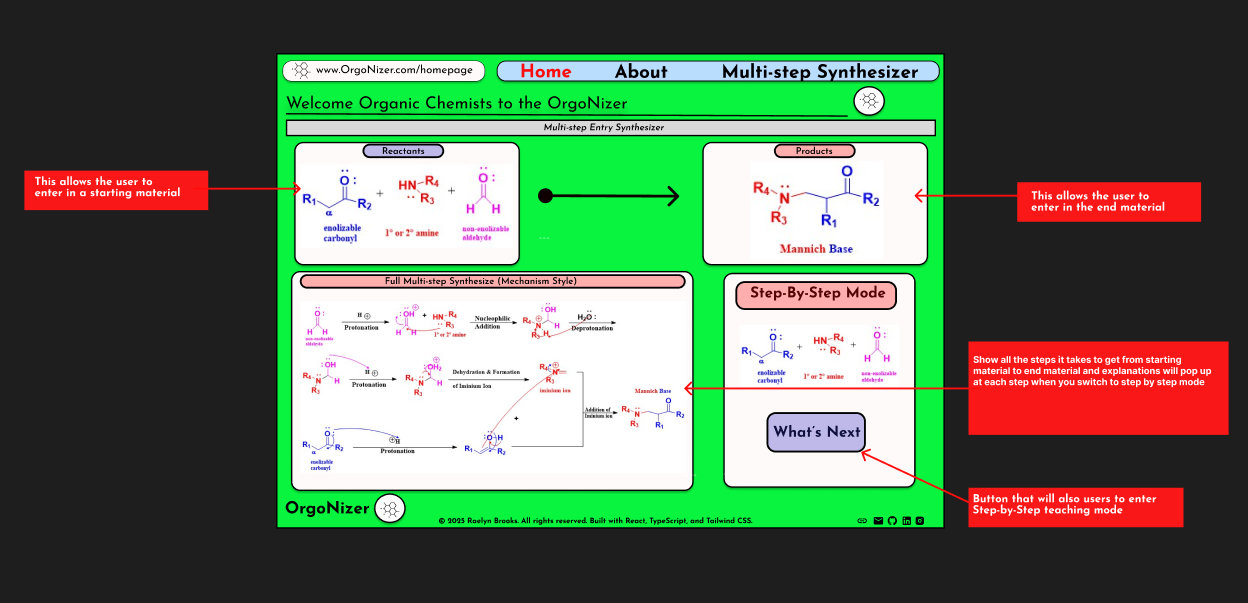
\includegraphics[scale=0.50]{OrgoNizerJuniorIs.png}
    \caption{Proposed system architecture for the Multistep Synthesis Tool. 
    The interface allows users to input a starting material and target molecule 
    either by name or drawing. A decision tree engine generates possible 
    multistep synthesis pathways, with constraints applied to ensure chemical 
    validity and explanations provided at each step.}
    \label{fig:orgonizer-architecture} % Unique label for referencing
\end{figure}



\newpage
\section*{Appendix}
Planned features for the Multistep Synthesis Tool for Organic Chemistry include:
\begin{itemize}
	\item Load dataset of organic molecules and reactions. (Existing dataset with names, structures, reactions, and reaction conditions.)
	\item Input molecule by name or drawing. (Name of a starting material or target molecule and convert it into a structured chemical format.)
	\item Confirm and display input molecules. (Show the user the structure of the input molecule to confirm correctness.)
	\item Search function for molecules. (Add a search feature that lets users find molecules, reagents, or intermediates within the dataset for use in pathway.)
	\item Generate single-step transformations. (Build logic to propose valid one-step transformations from the starting material toward the target product.)
	\item Generate multistep synthesis pathways. (Use decision trees and constraint satisfaction to create multistep synthesis routes from starting material to target product.)
	\item Step-by-step walkthrough mode with explanations. (Create an interactive mode where the user can walk through each reaction step with explanations of the reagents, conditions, and reasoning.)
	\item Constraint enforcement on pathways. (Implement rule checks that block or flag invalid or chemically impossible steps, with clear error explanations.)
	\item Store all molecules and reactions in a database. (MongoDB or similar NoSQL database to efficiently store and query chemical data.)
	\item User interface for interaction. (Simple web or desktop UI to input molecules, view structures, and navigate synthesis pathways.)
	\item Test on actual synthesis problems. (Use real-world synthesis problems from textbooks or literature to validate the tool's effectiveness.)
	
	\title{\textbf{Stretch Goals:}}
	\item Instructor problem mode (create custom synthesis problems for students to solve)
	\item Integrate cheminformatics library (e.g., RDKit) for advanced molecule handling and visualization
	\item User accounts and progress tracking (save synthesis attempts and scores over time)
	\item Machine learning suggestion layer (use ML models to suggest likely reagents or pathways based on historical data)
\end{itemize}


\bibliographystyle{acm}
\bibliography{bibliography.bib}

\end{document}
